

\documentclass[letterpaper, 10 pt, conference]{ieeeconf} 
\IEEEoverridecommandlockouts            
\overrideIEEEmargins
\usepackage[utf8]{inputenc}
\usepackage[T1]{fontenc}
\usepackage[makeroom]{cancel}
\pagenumbering{roman}
\usepackage{graphicx}
\usepackage{multirow}
\usepackage{amssymb}
\usepackage{amsmath}
\usepackage{physics}
\usepackage{amsmath}
\usepackage{amssymb}
\usepackage{cite}

\title{\LARGE \bf
Compact broadband filters in passive silicon photonics using cascaded optical ring resonators
}


\author{Daniel Hutama$^{1}$ % <-this % stops a space
\thanks{$^{1}$The Photonic Systems Group, Department of Electrical and Computer Engineering, McGill University, 3480 University St. room 753, Montreal, Quebec H3A 2A7}
}


\begin{document}



\maketitle
\thispagestyle{empty}
\pagestyle{empty}


%%%%%%%%%%%%%%%%%%%%%%%%%%%%%%%%%%%%%%%%%%%%%%%%%%%%%%%%%%%%%%%%%%%%%%%%%%%%%%%%
\begin{abstract}


We report on experimental and simulation results pertaining to the filter response of single and cascaded optical ring resonators (ORRs) in silicon photonics (SiP). Using three-dimensional finite-different time-domain simulations, we identify appropriate design parameters for our ORR devices. Using these parameters, we design a layout for experimental verification on a fabricated device. We show that ORRs can be used to implement compact optical filters with high extinction ratios. In addition, we show that cascaded ORRs can be used to achieve a broadband transmission spectrum in SiP in the 1500-1600 nm range. Using single ORRs, we achieved a filter response of $1927381238$ with $3259$. Our cascaded ORR device achieved a filter response of $0374$ with $2352354$.
\end{abstract}


%%%%%%%%%%%%%%%%%%%%%%%%%%%%%%%%%%%%%%%%%%%%%%%%%%%%%%%%%%%%%%%%%%%%%%%%%%%%%%%%
\section{Introduction}

Silicon photonics (SiP) is a rapidly evolving field due to its compatibility with existing CMOS fabrication processes, which allows electronic components to be integrated on the same chip as photonic devices. Developments in SiP devices show promise for new applications in several areas, such as sensing, communications, and computing. Such applications often require compact switch and filter components capable of providing large extinction ratios in a desired wavelength range. One way of implementing such devices is using optical ring resonators (ORRs), which provide a more compact and wavelength-selective alternative to larger Mach Zehnder-based devices \cite{SIPORR}. 

This paper is structured as follows: First, we briefly present theoretical insight into the operation of passive ORR devices. We then present three-dimensional finite-difference time-domain (3D FDTD) simulations to identify appropriate design parameters, and to demonstrate the expected thermal behavior of the devices. Following this, we present the fabricated design and discuss the experimental results.

\subsection*{Optical Ring Resonators}

Optical ring resonators are formed by a looped optical waveguide, as shown in Figure \ref{fig:1}. Light from a nearby straight waveguide couples into the resonator, with the coupling strength determined by several parameters, such as the gap distance, effective index, and wavelength. An ORR is said to be ''on resonance'' when the propagating wavelength fits an integer number of times inside the optical length of the ring cavity. In other words,
\begin{equation}
    \lambda_\text{res} = \frac{2\pi R n_\text{eff}}{m}, \qquad m \in \mathbb{Z}^+,
    \label{eq:lamdares}
\end{equation}
where $R$ is the radius of the ring and $n_\text{eff}$ is the effective index of the guided mode. When an input waveguide is placed in close proximity to an ORR, the incoming signal will selectively couple from the waveguide to the resonator, depending on if the wavelength of the signal satisfies the resonance condition of the ORR.

\begin{figure}[!ht]
    \centering
    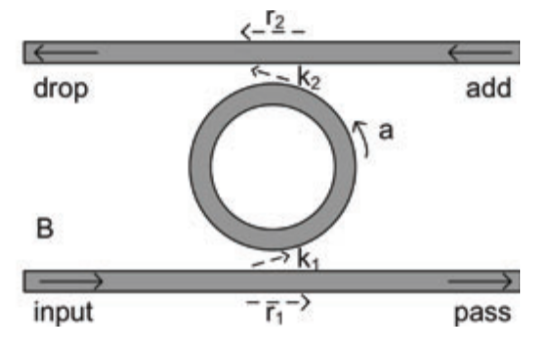
\includegraphics[width = 0.45\textwidth]{add_drop_RR.png}
    \caption{From \cite{SIPORR}. Schematic of an add-drop ring resonator. The self-coupling ratios ($r_i$) and cross-coupling ratios ($k_i$) are such that $r_i^2+k_i^2=1$.}
    \label{fig:1}
\end{figure} 

Using coupled-mode theory \cite{photonicdevices}, one can find the transmission at the pass and drop ports for the double-bus ring resonator shown in Figure \ref{fig:1}:
\begin{align}
    T_p &= \dfrac{r_2^2a^2-2r_1r_2a\cos\phi + r_1^2}{1-2r_1r_2a\cos\phi + (r_1r_2a)^2} \\
    T_d &= \dfrac{(1-r_1^2)(1-r_2^2)a}{1-2r_1r_2a\cos\phi + (r_1r_2a)^2},
\end{align}
where $\phi$ is the single-pass phase shift, given by $\phi = \beta \cdot (2\pi R)$, where $\beta$ is the propagation constant of the circulating mode. In addition, $a = \exp(-\alpha \cdot 2\pi R/2)$, where $\alpha$ is the power attenuation coefficient $[1/$cm$]$.

Under resonant conditions corresponding to $\phi = 2\pi m$, the transmission at the pass port reduces to 
\begin{equation}
    T_p^{\text{res}} = \dfrac{(r_2a-r_1)^2}{(1-r_1r_2a)^2},
    \label{eq:crit}
\end{equation}
with critical coupling occurring for $r_2a=r_1$, at which point the transmission to the pass port is $0$. The double-bus ring resonator can thus act as both a notch filter (at the pass port) and switch (to the drop port) at the resonant wavelength. With this theory in mind, we proceed with simulations to identify the appropriate design parameters to achieve critical coupling.


\section{Simulation}
\subsection*{Double-bus Resonators}
In order to achieve critical coupling, we must identify the appropriate self-coupling and cross-coupling ratios, $r_i$ and $k_i$, as shown in Figure \ref{fig:1}. From equation \eqref{eq:crit}, critical coupling for the double-bus resonator occurs when $r_2a = r_1$. To simplify our analysis, we assume that the loss is negligible ($a\approx 1)$, such that the critical condition is approximately met when the cross-coupling ratios are symmetric, i.e. $|r_1| = |r_2|$ and $|k_1| = |k_2|$. We chose a target $k=0.5$, which is done primarily to make our analysis for cascaded ring resonators easier. To find the gap distance between the straight waveguide and ring that corresponds to $k=0.5$, we performed a series of 3D FDTD simulations, like the one shown in Figure \ref{fig:sim3d}.

\begin{figure}[!ht]
    \centering
    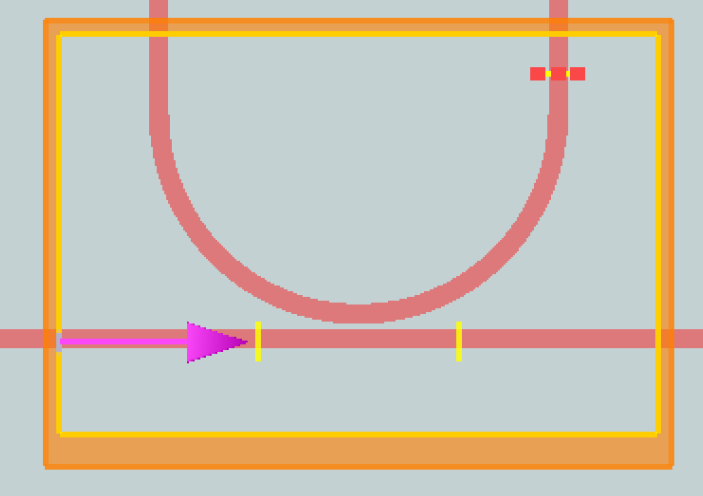
\includegraphics[width = 0.4\textwidth]{gapdist.png}
    \caption{3D FDTD simulation setup to identify gap to coupling parameter relationship. Input light is denoted with the magenta arrow. The output at the drop port is measured using a power meter, which measures the power coupling ratio $k =\dfrac{\frac{1}{2}\int_\mathcal{S}\text{real}(\vec{P})\cdot d\vec{A}}{\text{source power}}$, where $\mathcal{S}$ is the surface of a planar power monitor, $\vec{P}$ is the Poynting vector normal to $\mathcal{S}$, and $d\vec{A}$ is the surface normal element. }
    \label{fig:sim3d}
\end{figure} 

The simulated waveguides have cross-section dimensions of $220$ x $500$ nm, which are the same as the fabricated waveguides. The half-ring radius is $5$ $\mu$m. We performed five simulations, with the parameter of interest being the gap distance. By varying the gap from 100 nm to 200 nm in increments of $25$ nm, we observed a $\Delta k$ of $0.36$, as shown in Table \ref{tab:sim}. 

\begin{table}[!ht]
\centering
\caption{Simulated cross-coupling coefficient vs. gap distance.}
\begin{tabular}{|c|c|}
\hline
\textbf{Gap Distance} & \textbf{$k$} \\ \hline
100 nm & 0.7539 \\ \hline
125 nm & 0.6473 \\ \hline
150 nm & 0.5583 \\ \hline
175 nm & 0.4698 \\ \hline
200 nm & 0.3941 \\ \hline
\end{tabular}
\label{tab:sim}
\end{table}



\subsection*{Double-bus Resonator Temperature Dependence} 
Although temperature dependence is not experimentally verified, we simulated the spectral response of the double-bus resonators under different temperatures. As shown in Figure \ref{fig:temp}, the resonant wavelengths experience a blue-shift of approximately 4.5 nm when the temperature is increased from $270$ K to $300$ K.

\begin{figure}[!ht]
    \centering
    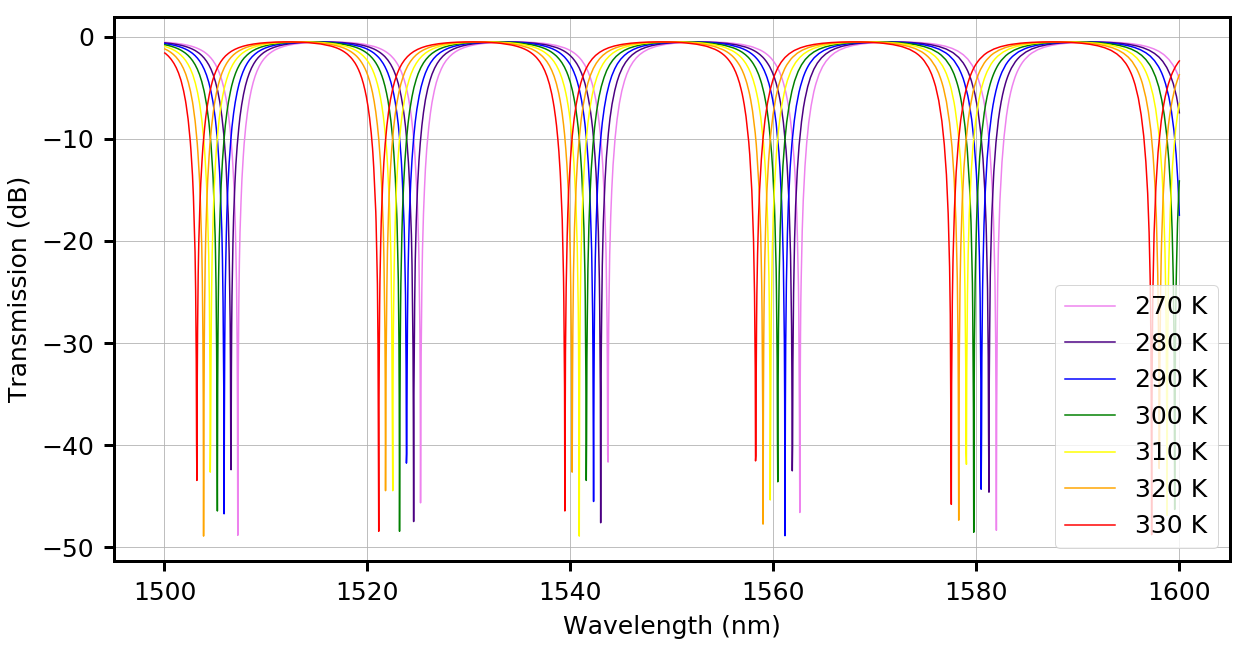
\includegraphics[width = 0.485\textwidth]{Temp_dependence.png}
    \caption{Simulated transmission spectrum of a double-bus ring resonator with symmetric coupling coefficients of $k = 0.5$ with temperatures ranging from $270$ K to $330$ K in increments of $10$ K.}
    \label{fig:temp}
\end{figure} 

\subsection*{Cascaded Resonators}

\section{Experiment}

After obtaining the appropriate design parameters from simulation, we designed a layout of the test structures for fabrication, as shown in figure \ref{fig:layout}. The layout includes five double-bus ring resonators with varying gap distances. In addition, the there are two cascaded ring resonator structures, with differing gap distances between the outer rings and straight waveguides. 

\begin{figure}[!ht]
    \centering
    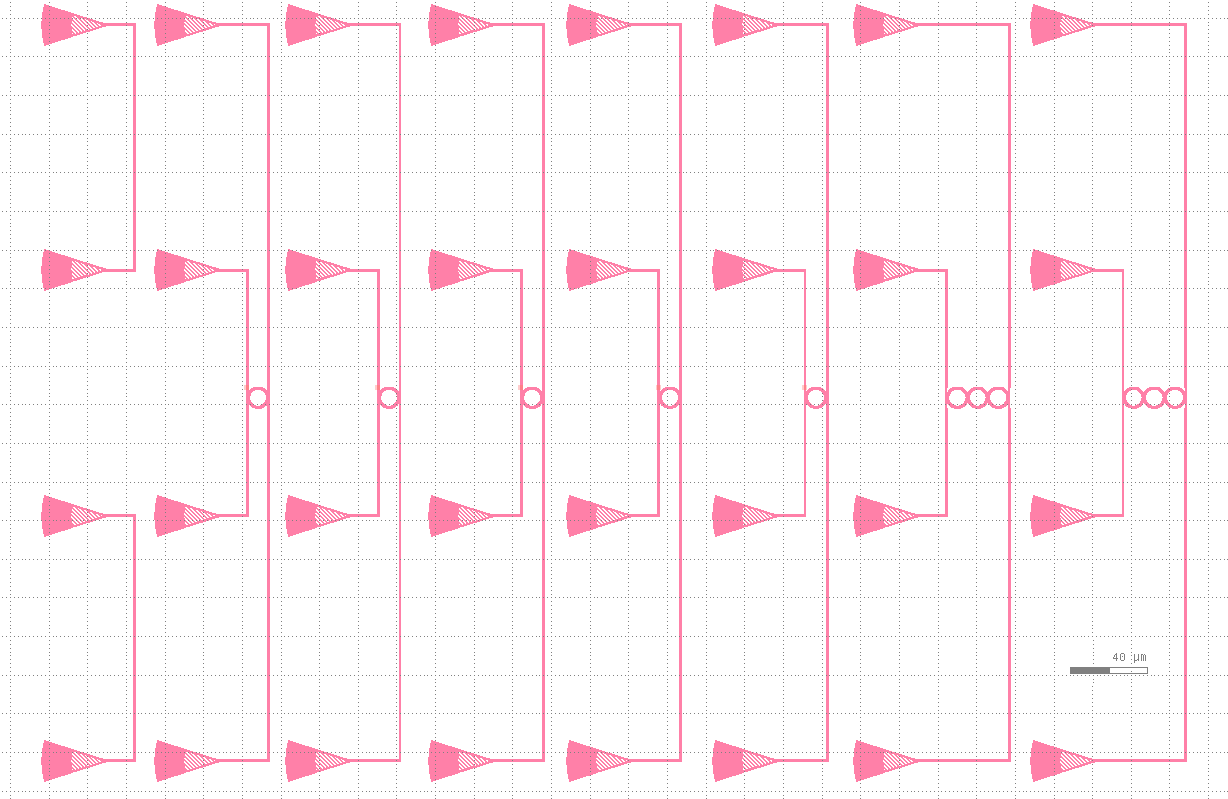
\includegraphics[width = 0.485\textwidth]{layout.png}
    \caption{Device layout submitted for fabrication at Applied Nanotools. From left to right: Loopback structures (x2) to isolate grating coupler response. Following this are five 5-$\mu$m radius rings with gap distances of 100 nm, 125 nm, 150 nm, 175 nm, and 200 nm. The final two structures are the cascaded 5-$\mu$m ring devices. The cascaded structure on the left has gaps of $115$ nm and $175$ nm, respectively, to the left and right of the middle ring, and a symmetric $175$ nm gap from the outer rings to the straight waveguides. The rightmost device is similar, but with $150$ nm gaps between the outer rings and straight waveguides.}
    \label{fig:layout}
\end{figure} 

Light is coupled in and out of the chip via vertical grating couplers (VGCs) designed for TE mode operation at $-31^\circ$ \cite{VGC}. To isolate the spectral response of the VGCs used in the experiment from the response of the test structures, we included two test devices which are simple input-output couplers connected by a strip waveguide. The response of the couplers are averaged, and fourth order polynomial is used to model the VGC response. The modeled VGC response is then subtracted from the spectral response of all test devices. 


\section{Conclusion}

temperature tunability





\bibliographystyle{IEEEtran}
\bibliography{mybib}


\end{document}
